\documentclass{beamer}
%
% Choose how your presentation looks.
%
% For more themes, color themes and font themes, see:
% http://deic.uab.es/~iblanes/beamer_gallery/index_by_theme.html
%
\mode<presentation>
{
  \usetheme{default}      % or try Darmstadt, Madrid, Warsaw, ...
  \usecolortheme{default} % or try albatross, beaver, crane, ...
  \usefonttheme{default}  % or try serif, structurebold, ...
  \setbeamertemplate{navigation symbols}{}
  \setbeamertemplate{caption}[numbered]
} 

\usepackage[english]{babel}
\usepackage[utf8x]{inputenc}

\title[Layer-wise Relevance Propagation (LRP) algorithm]{Layer-wise Relevance Propagation (LRP)\\Machine Learning for Health Informatics}
\author{Anna Saranti}
\institute{Holzinger Group hci-kdd.org}
\date{26.03.2019}

\begin{document}

\begin{frame}
  \titlepage
  
  \begin{figure}[ht]
	\centering
    
\includegraphics[width=3cm, height=3.5cm]{figures/HddKciLogo}
	\label{fig:HddKciLogo}
  \end{figure}
  
\end{frame}

% --------------------------------------------------------------------------------------------------
\begin{frame}{Outline}
  \tableofcontents
\end{frame}

%%%%%%%%%%%%%%%%%%%%%%%%%%%%%%%%%%%%%%%%%%%%%%%%%%%%%%%%%%%%%%%%%%%%%%%%%%%%%%%%%%%%%%%%%%%%%%%%%%%%
%%%%%%%%%%%%%%%%%%%%%%%%%%%%%%%%%%%%%%%%%%%%%%%%%%%%%%%%%%%%%%%%%%%%%%%%%%%%%%%%%%%%%%%%%%%%%%%%%%%%
%%%%%%%%%%%%%%%%%%%%%%%%%%%%%%%%%%%%%%%%%%%%%%%%%%%%%%%%%%%%%%%%%%%%%%%%%%%%%%%%%%%%%%%%%%%%%%%%%%%%
\section{Taylor decomposition}

\begin{frame}{Taylor Decomposition}

\begin{itemize}
  \item Taylor expansion of a function $f(x)$ at point $a$: \\
  $f(x) = f(a) + \frac{f'(a)}{1!}(x-a) + \frac{f''(a)}{2!}(x-a)^2 + \frac{f'''(a)}{3!}(x-a)^3 + \cdots$
\end{itemize}

\begin{itemize}
  \item Classification (output) $f(\mathbf{x})$ of input $\mathbf{x}$ (1st order only): \\
  $f(\mathbf{x}) = f(\tilde{\mathbf{x}}) + \Bigg( \frac{\partial f}{\partial \mathbf{x}} \biggr\rvert_{\mathbf{x} = \tilde{\mathbf{x}}} \Bigg)^T
  (\mathbf{x} - \tilde{\mathbf{x}}) + \epsilon $ \\
  $0 + \sum_p \underbrace{\frac{\partial f}{x_p} \biggr\rvert_{\mathbf{x} = \tilde{\mathbf{x}}} (x_p - \tilde{x}_p)}_\text{$R_p(\mathbf{x})$} + \epsilon  $ \\
  where $p$ is the index of the pixel.
  \item Find a neighbouring point $\tilde{\mathbf{x}}$, for which $f(\tilde{\mathbf{x}}) = 0$ 
  \item $\sum_j R_j = \Bigg( \frac{\partial (\sum_j R_j)}{\partial{\{x_i\}}}\biggr\rvert_{\partial \{\tilde{x}_i\} } \Bigg)^T (\{x_i\} - \{\tilde{x}_i\}) + \epsilon = $ \\ $\sum_i \sum_j \frac{\partial R_j}{\partial x_i}\biggr\rvert_{\partial \{\tilde{x}_i\} } (x_i - \tilde{x}_i) + \epsilon $
\end{itemize}

\end{frame}

% --------------------------------------------------------------------------------------------------
\begin{frame}{Pixel-wise decomposition of a function}

\begin{itemize}
  \item Goal: redistribute the neural network output onto the input variables; the relevance $R_j$ to lower-level relevances $\{R_i\}$
  \item How to choose the neighbouring point $\tilde{x}$ ?
  \item Similar image, object not recognizable from the classifier - \\
  hence the output $f(\tilde{\mathbf{x}}) = 0$
\end{itemize}

\begin{figure}[ht]
	\centering
    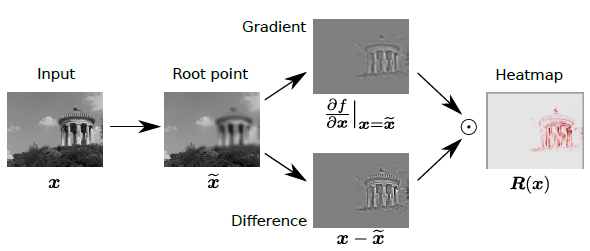
\includegraphics[width=8cm, height=3.5cm]{figures/choose_x}
	\label{fig:ChooseX}
\end{figure}

\end{frame}
% --------------------------------------------------------------------------------------------------
\begin{frame}{Properties}

\begin{itemize}
  \item Conservation: $\forall \mathbf{x}: f(\mathbf{x}) = \sum_p R_p(\mathbf{x})$ \\
  $\sum_j R_j = \sum_i R_i$ ($i$ and $j$ are layers)
  \item Positivity: $\forall \mathbf{x}, p: R_p(\mathbf{x}) \geq 0$
\end{itemize}

\vspace{20px}

\begin{itemize}
  \item Rectified Linear Unit:
\end{itemize}
\begin{figure}[ht]
	\centering
    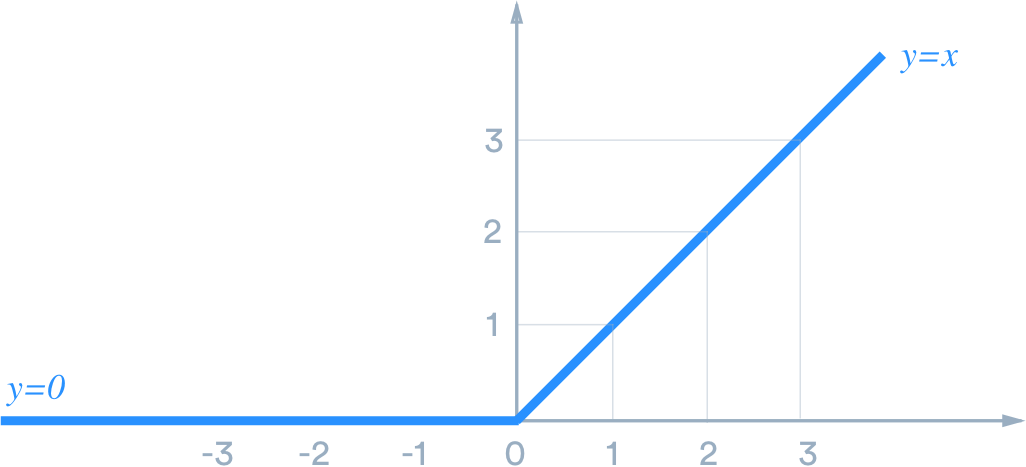
\includegraphics[width=8cm, height=3.5cm]{figures/ReLU}
	\label{fig:ReLU}
\end{figure}

\end{frame}
% --------------------------------------------------------------------------------------------------
\section{Example}
\begin{frame}{Example (1/2)}

\begin{figure}[ht]
	\centering
    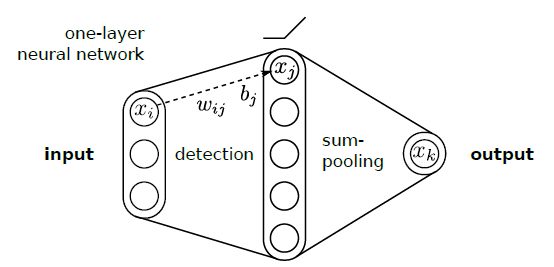
\includegraphics[width=10cm, height=5cm]{figures/one_layer_network}
	\label{fig:OneLayerNetwork}
\end{figure}

\begin{itemize}
\item $x_j = max(0, \sum_i x_i w_{ij} + b_j)$ (ReLU nonlinearity)
\item $x_k = \sum_j x_j$ (Sum pooling)
\end{itemize}

\end{frame}

% -------------------------------------------------------------------------------------------------
\begin{frame}{Example (2/2)}

$R_k$ of output layer: Total relevance that must be backpropagated:
\begin{itemize}
\item $R_k = x_k = \sum_j x_j$ 
\end{itemize}

$R_j$ of hidden layer: Taylor decomposition on $\{ \tilde{x}_j \} = 0$:
\begin{itemize}
\item $R_j = R_k(\tilde{\mathbf{x}}) + \frac{\partial R_k}{\partial x_j} \biggr\rvert_{\{ \tilde{x}_j \}} \cdot (x_j - \tilde{x}_j) = x_j = max(0, \sum_i x_i w_{ij} + b_j)$ \\
\item For which $\tilde{\mathbf{x}}$ is $R_k(\tilde{\mathbf{x}}) = 0$? \\ 
Since ReLU ensures that $\{ \forall j: \tilde{x_j} \geq 0 \}$ and \\ 
$\frac{\partial R_k}{\partial x_j} = \frac{\partial \sum_j x_j}{\partial x_j} = 1$
\end{itemize}

$R_i$ of input layer: 
\begin{itemize}
\item $R_i = \sum_j \frac{\partial R_j}{\partial x_i} \biggr\rvert_{\{ \tilde{x}_i \}^{(j)}} \cdot (x_i - \tilde{x}_i^{(j)})$
\item $R_i = \sum_j \frac{w_{ij}^2}{\sum_{i'} w_{i'j}^2} R_j$ 
\end{itemize}

\end{frame}

%%%%%%%%%%%%%%%%%%%%%%%%%%%%%%%%%%%%%%%%%%%%%%%%%%%%%%%%%%%%%%%%%%%%%%%%%%%%%%%%%%%%%%%%%%%%%%%%%%%%
%%%%%%%%%%%%%%%%%%%%%%%%%%%%%%%%%%%%%%%%%%%%%%%%%%%%%%%%%%%%%%%%%%%%%%%%%%%%%%%%%%%%%%%%%%%%%%%%%%%%
%%%%%%%%%%%%%%%%%%%%%%%%%%%%%%%%%%%%%%%%%%%%%%%%%%%%%%%%%%%%%%%%%%%%%%%%%%%%%%%%%%%%%%%%%%%%%%%%%%%%
\section{Task description}

\begin{frame}{Task (1/2)}

The task contains two parts
\begin{enumerate}
\item Numerical task
	\begin{itemize}
		\item Use the equations above to compute numerically the relevance of all layers of the network depicted in the figure.
		\item Use your own weight values ($w_{ij}$), but think on weighting schemes that are typically used in neural networks.\\
		See \url{https://keras.io/initializers/}
		\item Verify that the conservation and positivity rules properties apply.
		\item Provide descriptions of the interpretations
	\end{itemize}
\item Programmatic task
	\begin{itemize}
		\item Install Python 3.5.+ and the relevant libraries.
		\item Provide descriptions of the interpretations of the relevance images with respect to the input images as well as their differences
	\end{itemize}
\end{enumerate}

\end{frame}
% -------------------------------------------------------------------------------------------------
\begin{frame}{Task (2/2)}

\begin{enumerate}
\item Python libraries
	\begin{itemize}
		\item \url{https://www.tensorflow.org/}, \url{https://mxnet.apache.org/}
		\item \url{https://keras.io/}
		\item \url{https://github.com/albermax/innvestigate}
		\item Run the \texttt{examples/readme\_code\_snippet.py} with any of the \texttt{.jpg} figures in the \texttt{examples/images} folder (line 37)
		\item Adapt line 54 to select a different analyzer
		\item Python IDE: \url{https://www.jetbrains.com/pycharm/}
	\end{itemize}
\end{enumerate}

\end{frame}

%%%%%%%%%%%%%%%%%%%%%%%%%%%%%%%%%%%%%%%%%%%%%%%%%%%%%%%%%%%%%%%%%%%%%%%%%%%%%%%%%%%%%%%%%%%%%%%%%%%%
%%%%%%%%%%%%%%%%%%%%%%%%%%%%%%%%%%%%%%%%%%%%%%%%%%%%%%%%%%%%%%%%%%%%%%%%%%%%%%%%%%%%%%%%%%%%%%%%%%%%
%%%%%%%%%%%%%%%%%%%%%%%%%%%%%%%%%%%%%%%%%%%%%%%%%%%%%%%%%%%%%%%%%%%%%%%%%%%%%%%%%%%%%%%%%%%%%%%%%%%%
\begin{frame}{Literature}

\begin{itemize}
	\item Montavon, Grégoire, et al. "Explaining nonlinear classification decisions with deep taylor decomposition." Pattern Recognition 65 (2017): 211-222.
\end{itemize}

\end{frame}

\end{document}